\section{Model dwukryterialny zysku i ryzyka}
\addcontentsline{toc}{section}{Model dwukryterialny zysku i ryzyka}

\subsection{Model zadania}
\addcontentsline{toc}{subsection}{Model zadania}
W ramach niniejszego zadania zastosowano model przedsiębiorstwa identyczny z tym wykorzystanym w pierwszej części analizy. 
Kryterium zysku jest nadal reprezentowane przez wartość oczekiwaną, która dla scenariuszy charakteryzujących się jednakowym 
prawdopodobieństwem wystąpienia jest równoważna wartości średniej. Kryterium ryzyka zostało zdefiniowane przy użyciu średniej 
różnicy Giniego, opisanej poniższą formułą:
\begin{equation}
\Gamma(\mathbf{x})=\frac{1}{2}\sum_{t'=1}^{T}\sum_{t"=1}^{T}\lvert r_{t'}(\mathbf{x})-r_{t"}(\mathbf{x})\rvert p_{t'}p_{t"}, 
\end{equation}
gdzie $r_{t'}(\mathbf{x})$ reprezentuje wartość zysku osiągniętą w scenariuszu $t'$, natomiast $p_{t}$ określa prawdopodobieństwo wystąpienia scenariusza $t$.

Wykorzystując notację zastosowaną w niniejszym projekcie, formula określająca miarę ryzyka przyjmuje następującą formę:
\begin{multline}
riskMeasureGini = \frac{1}{2}\cdot\sum_{t1 \in scenarios}\sum_{t2 \in scenarios} \lvert profit[t1]-profit[t2] \rvert \cdot \\ \frac{1}{numberOfScenarios} \cdot \frac{1}{numberOfScenarios} 
\end{multline}

\subsection{Model preferencji}
\addcontentsline{toc}{subsection}{Model preferencji}
Model preferencji oparto na minimalizacji ryzyka przy zadanym poziomie średniego zysku.
\begin{equation}
averageProfit<minimalAverageProfit
\end{equation}
\begin{equation}
minimize riskMeasureGini
\end{equation}
minimalAverageProfit stanowi dodatkowy parametr modelu. Pliki wdwr25406-3.dat i wdwr25406-3.mod i modelem zadania dwukryterialnego wyboru - 
pliki źródłowe przeznaczone dla solvera CPLEX. 

\subsection{Zbiór rozwiązań efektywnych w przestrzeni ryzyko-zysk}
\addcontentsline{toc}{subsection}{Zbiór rozwiązań efektywnych w przestrzeni ryzyko-zysk}
Na rysunku \ref{fig:profit-risk} przedstawiono krzywa efektywności w przestrzeni ryzyko-zysk. 
Punkty reprezentują rozwiązania efektywne 
uzyskane dla różnych poziomów wymaganego zysku. Ze względu na ograniczenia obliczeniowe, 
wygenerowano 20 równomiernie rozłożonych punktów,
przy czym każdy z nich opiera się na 30 scenariuszach. Ustalono limit czasowy działania solvera 
na 10 sekund dla pojedynczego rozwiązania (wydłużenie tego limitu przyniosło jedynie niewielką 
poprawę dokładności przy znacząco zwiększonym czasie obliczeń).
W plikach wdwr25406-3.dat oraz wdwr25406-3.mod znajdują się definicje parametrów i 
modelu wraz z implementacją dla solvera CPLEX. 
Wartości ekstremalne - maksymalny zysk oraz 
minimalne ryzyko - zostały zestawione w poniższej tabeli
\begin{figure}[H]
\centering
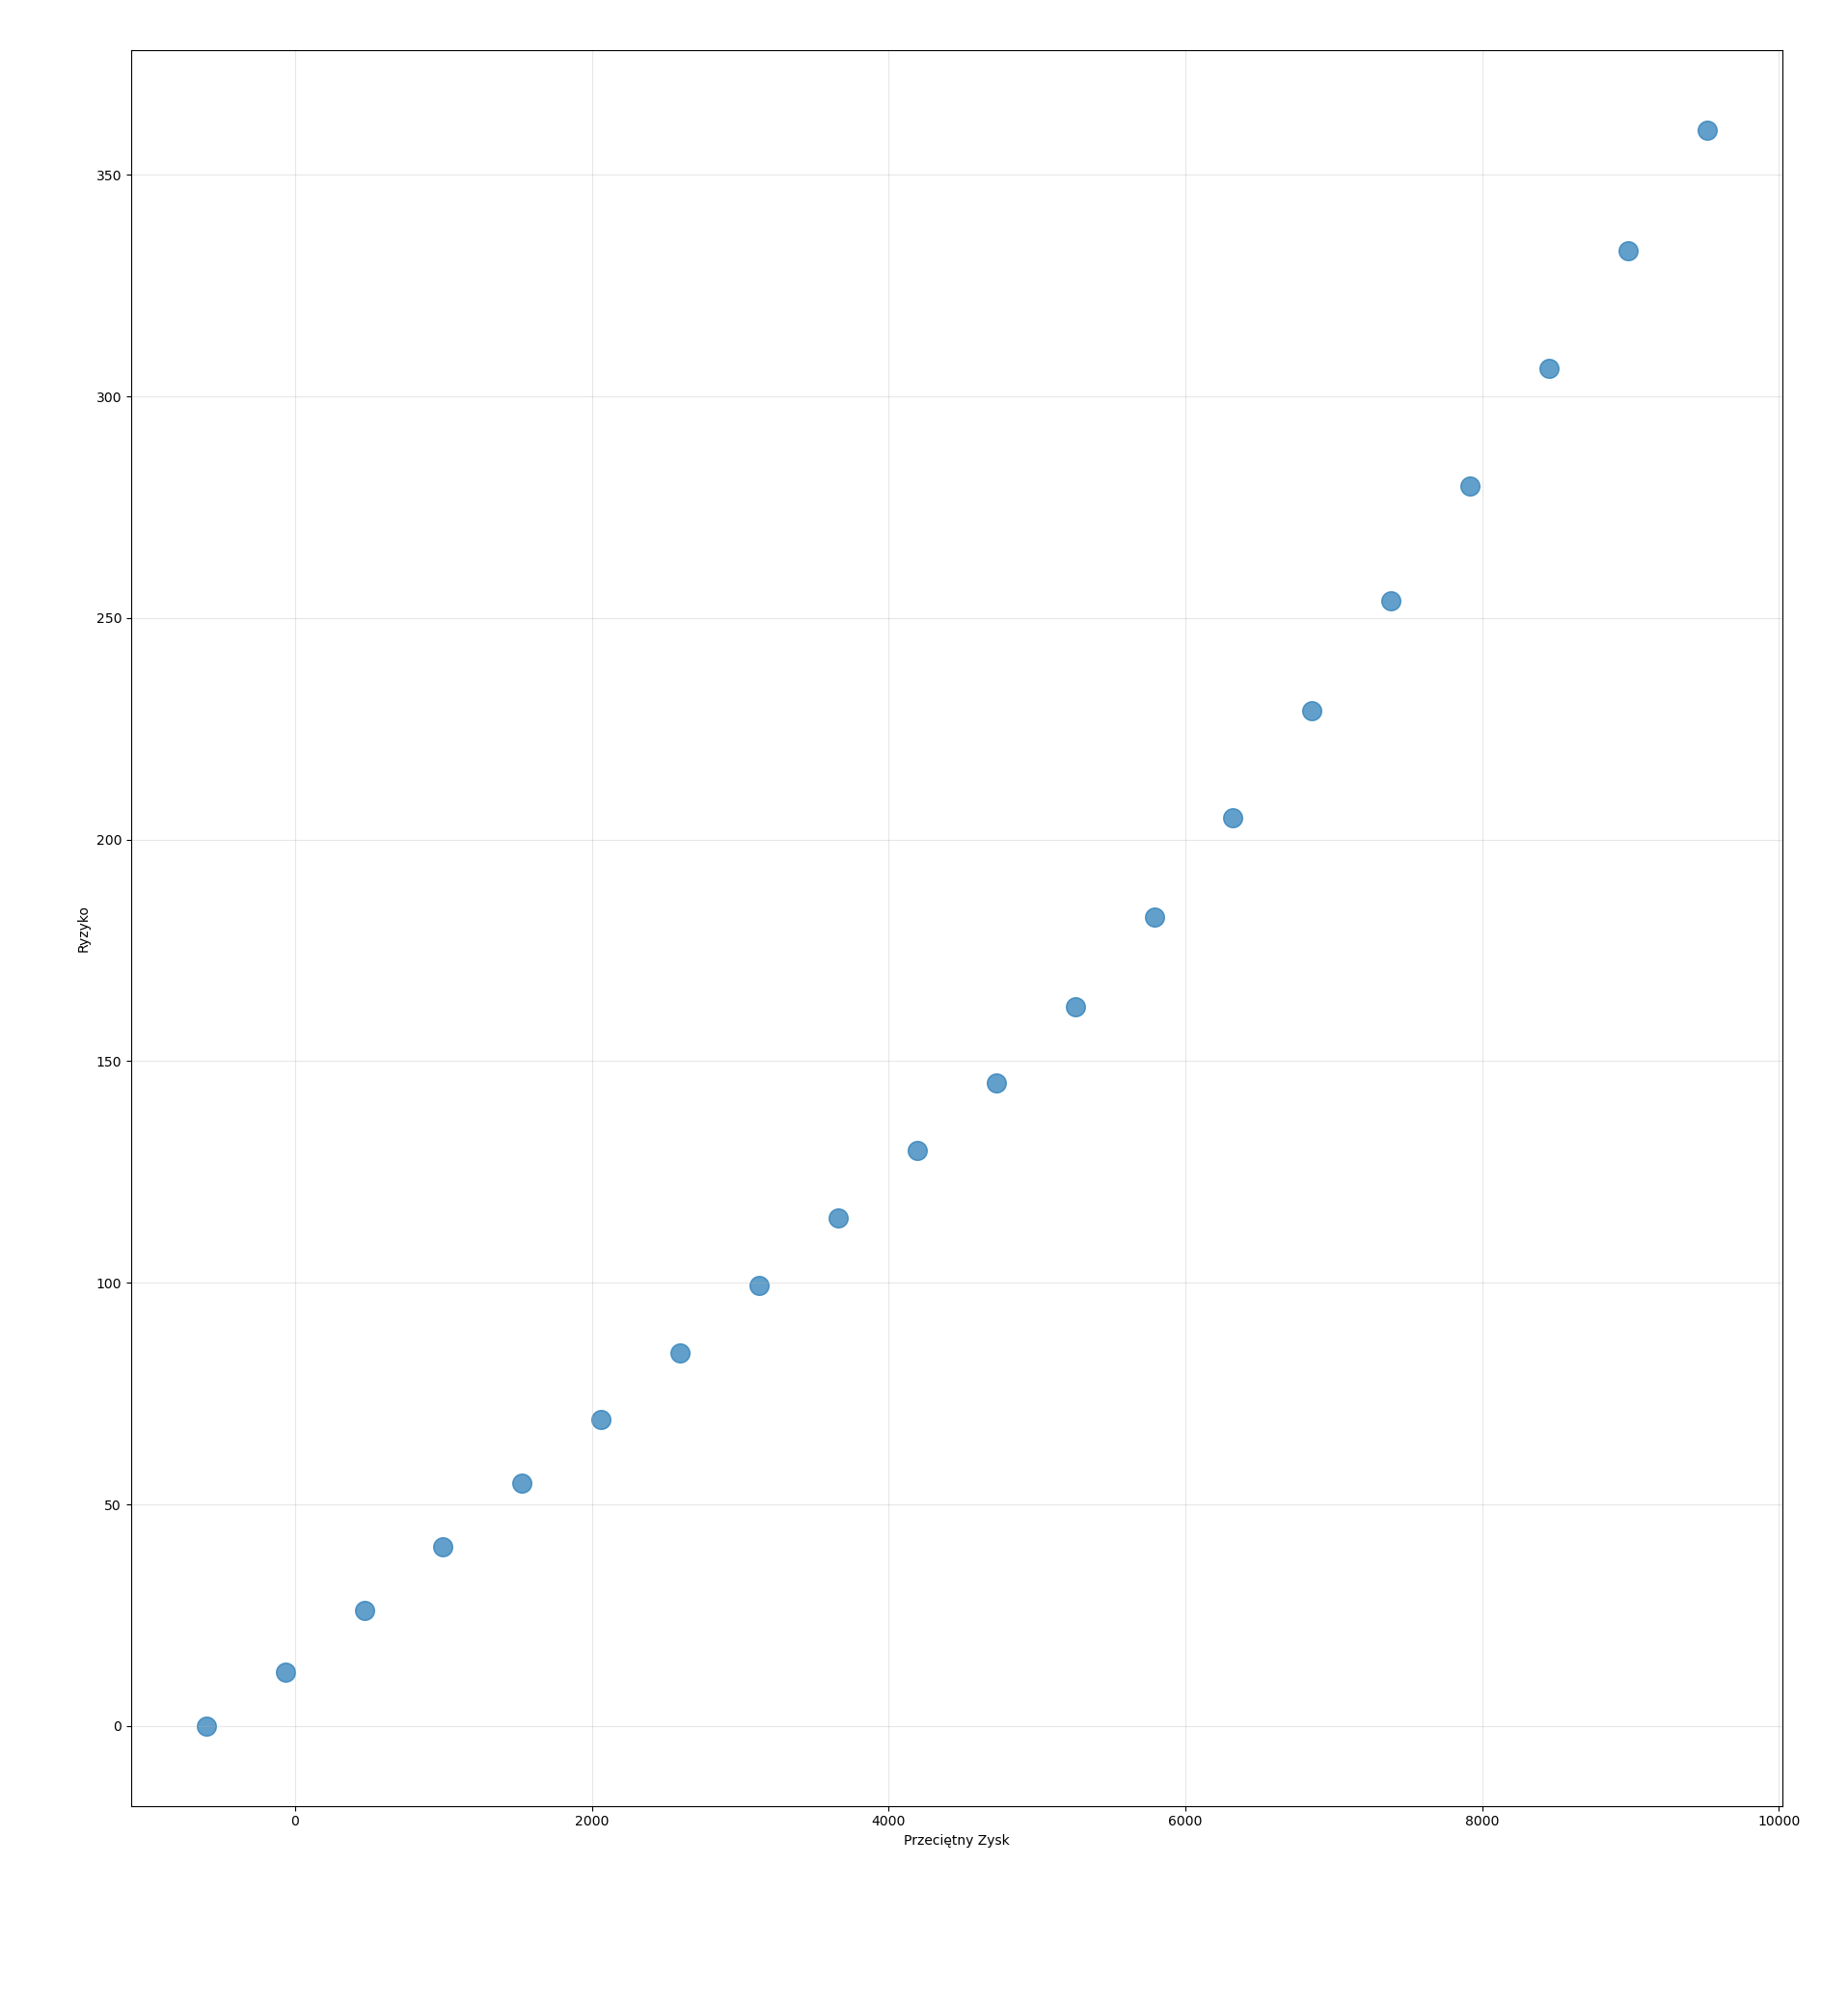
\includegraphics[width=0.8\textwidth]{graphics/ryzyko_zysk_wykres.png}
\caption{Obraz zbioru rozwiązań efektywnych w przestrzeni ryzyko-zysk}
\label{fig:profit-risk}
\end{figure}

\subsection{Rozwiązania efektywne minimalnego ryzyka i maksymalnego zysku}
\addcontentsline{toc}{subsection}{Rozwiązania efektywne minimalnego ryzyka i maksymalnego zysku}

\begin{table}[H]
\label{tab:min-max}
  \caption{Rozwiązania maksymalnego zysku i minimalnego ryzyka}
  \centering
  \begin{tabular}{l*{4}{c}}
  
  	\hline
              			& Miara zysku & Miara ryzyka \\
	\hline
	Maksymalizacja zysku	& 9515.80 zł & 360.18 zł \\
	Minimalizacja ryzyka   	& -600.00 zł & 0.0 zł \\ 
	\hline
	
	\end{tabular}
	\end{table}
	
Rozwiązanie zadania jednokryterialnego maksymalizacji zysku charakteryzuje się również maksymalizacją poziomu ryzyka, podczas gdy zadanie 
minimalizacji ryzyka bez nałożenia ograniczeń na poziom zysku prowadzi do ujemnego wyniku finansowego (straty) wynikającego z rezygnacji ze 
sprzedaży oraz ponoszenia kosztów utrzymania obligatoryjnych zapasów magazynowych.

\subsection{Dominacja stochastyczna wybranych rozwiązań efektywnych}
\addcontentsline{toc}{subsection}{Dominacja stochastyczna wybranych rozwiązań efektywnych}
Do weryfikacji relacji dominacji stochastycznej pierwszego rzędu (FSD) zostały wybrane 3 rozwiązania efektywne modelu: Scenariusze 1, 2 i 3,
Parametry charakteryzujące średni zysk i miarę ryzyka dla analizowanych rozwiązań przedstawiono w tabeli \ref{tab:abc}. 
Implementacja parametrów oraz modelu została zawarta w plikach wdwr25406-4.dat i wdwr25406-4.mod - skrypty przeznaczone dla solvera CPLEX 
służące do generowania informacji o zysku i ryzyku w ramach poszczególnych scenariuszy.

\begin{table}[H]
  \label{tab:abc}
  \caption{Scenariusze wybrane do analizy dominacji FSD}
  \centering
  \begin{tabular}{lccc}
  	\hline
              			& 1 & 2 & 3 \\
	\hline
	Ograniczenie minimalnego zysku	& 8450.97 zł & 8983.38 zł & 9515.79 zł\\
	Średni zysk   	& 8451.02 zł & 8983.40 zł & 9515.80 zł\\
	Miara ryzyka   	& 306.38 zł & 332.93 zł & 360.18 zł\\ 
	\hline
	\end{tabular}
\end{table}

Aby określić relacje dominacji między wybranymi rozwiązaniami w kontekście FSD, zbudowano odwrotne dystrybuanty 
dla obydwu analizowanych kryteriów. Rysunek \ref{fig:FSD-profit} prezentuje odwrotną dystrybuantę rozkładu średniego 
zysku w poszczególnych scenariuszach dla trzech wybranych rozwiązań efektywnych. Z analizy wykresu wynika, 
że rozwiązanie dla scenariusza 3 przewyższa rozwiązania scenariusza 1 i 2 w kontekście dominacji stochastycznej pierwszego rzędu, 
oznaczając, że dla każdego scenariusza wartość zysku osiągana przez decyzję 3 jest wyższa niż 
odpowiadające jej wartości dla decyzji 1 i 2. Jednocześnie rozwiązanie 2 dominuje nad rozwiązaniem 1
w sensie dominacji stochastycznej pierwszego rzędu.

\begin{figure}[H]
\centering
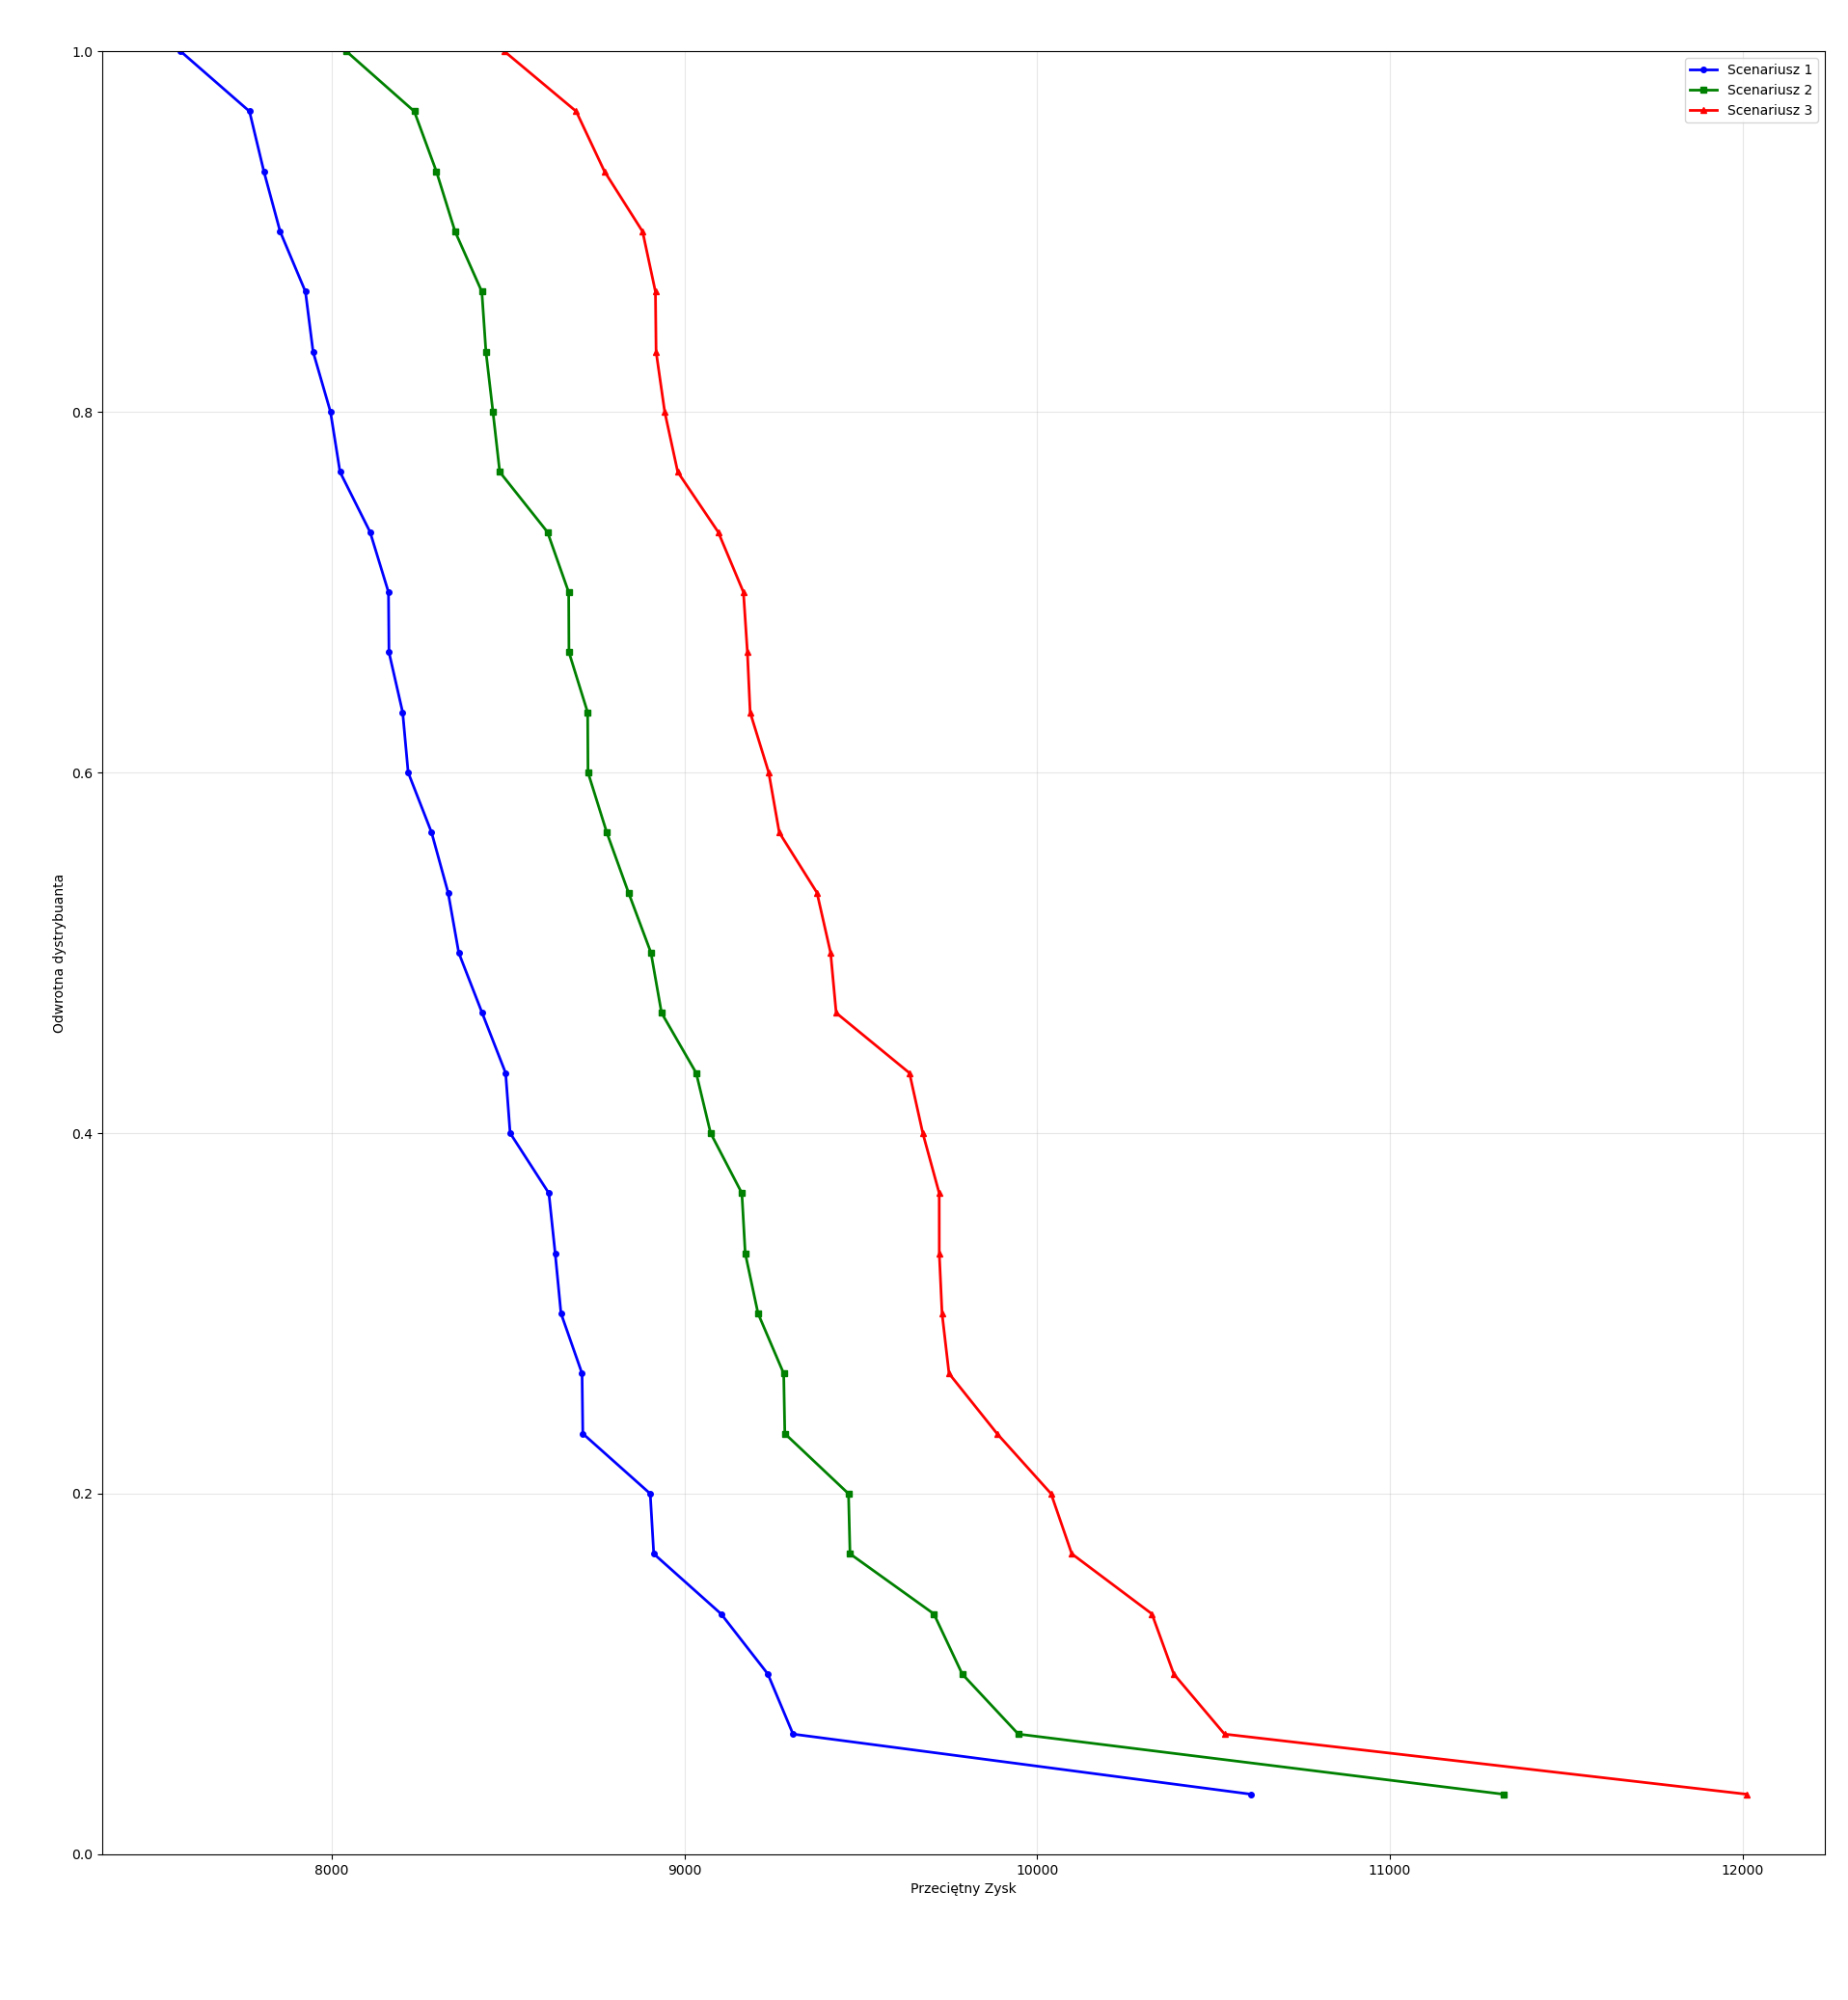
\includegraphics[width=\textwidth]{graphics/zysk_dystrybuanta.png}
\caption{Odwrotna dystrybuanta rozkładu średniego zysku między scenariuszami}
\label{fig:FSD-profit}
\end{figure}
Rysunek \ref{fig:FSD-risk} prezentuje odwrotną dystrybuantę rozkładu średniej różnicy Giniego jako miary ryzyka dla 
tych samych trzech rozwiązań efektywnych. W zakresie miary ryzyka rozwiązanie 1 charakteryzuje się dominacją 
nad rozwiązaniami 2 i 3, rozwiązanie 2 wykazuje również jednoznaczną dominację względem rozwiązania 3. 

\begin{figure}[H]
\centering
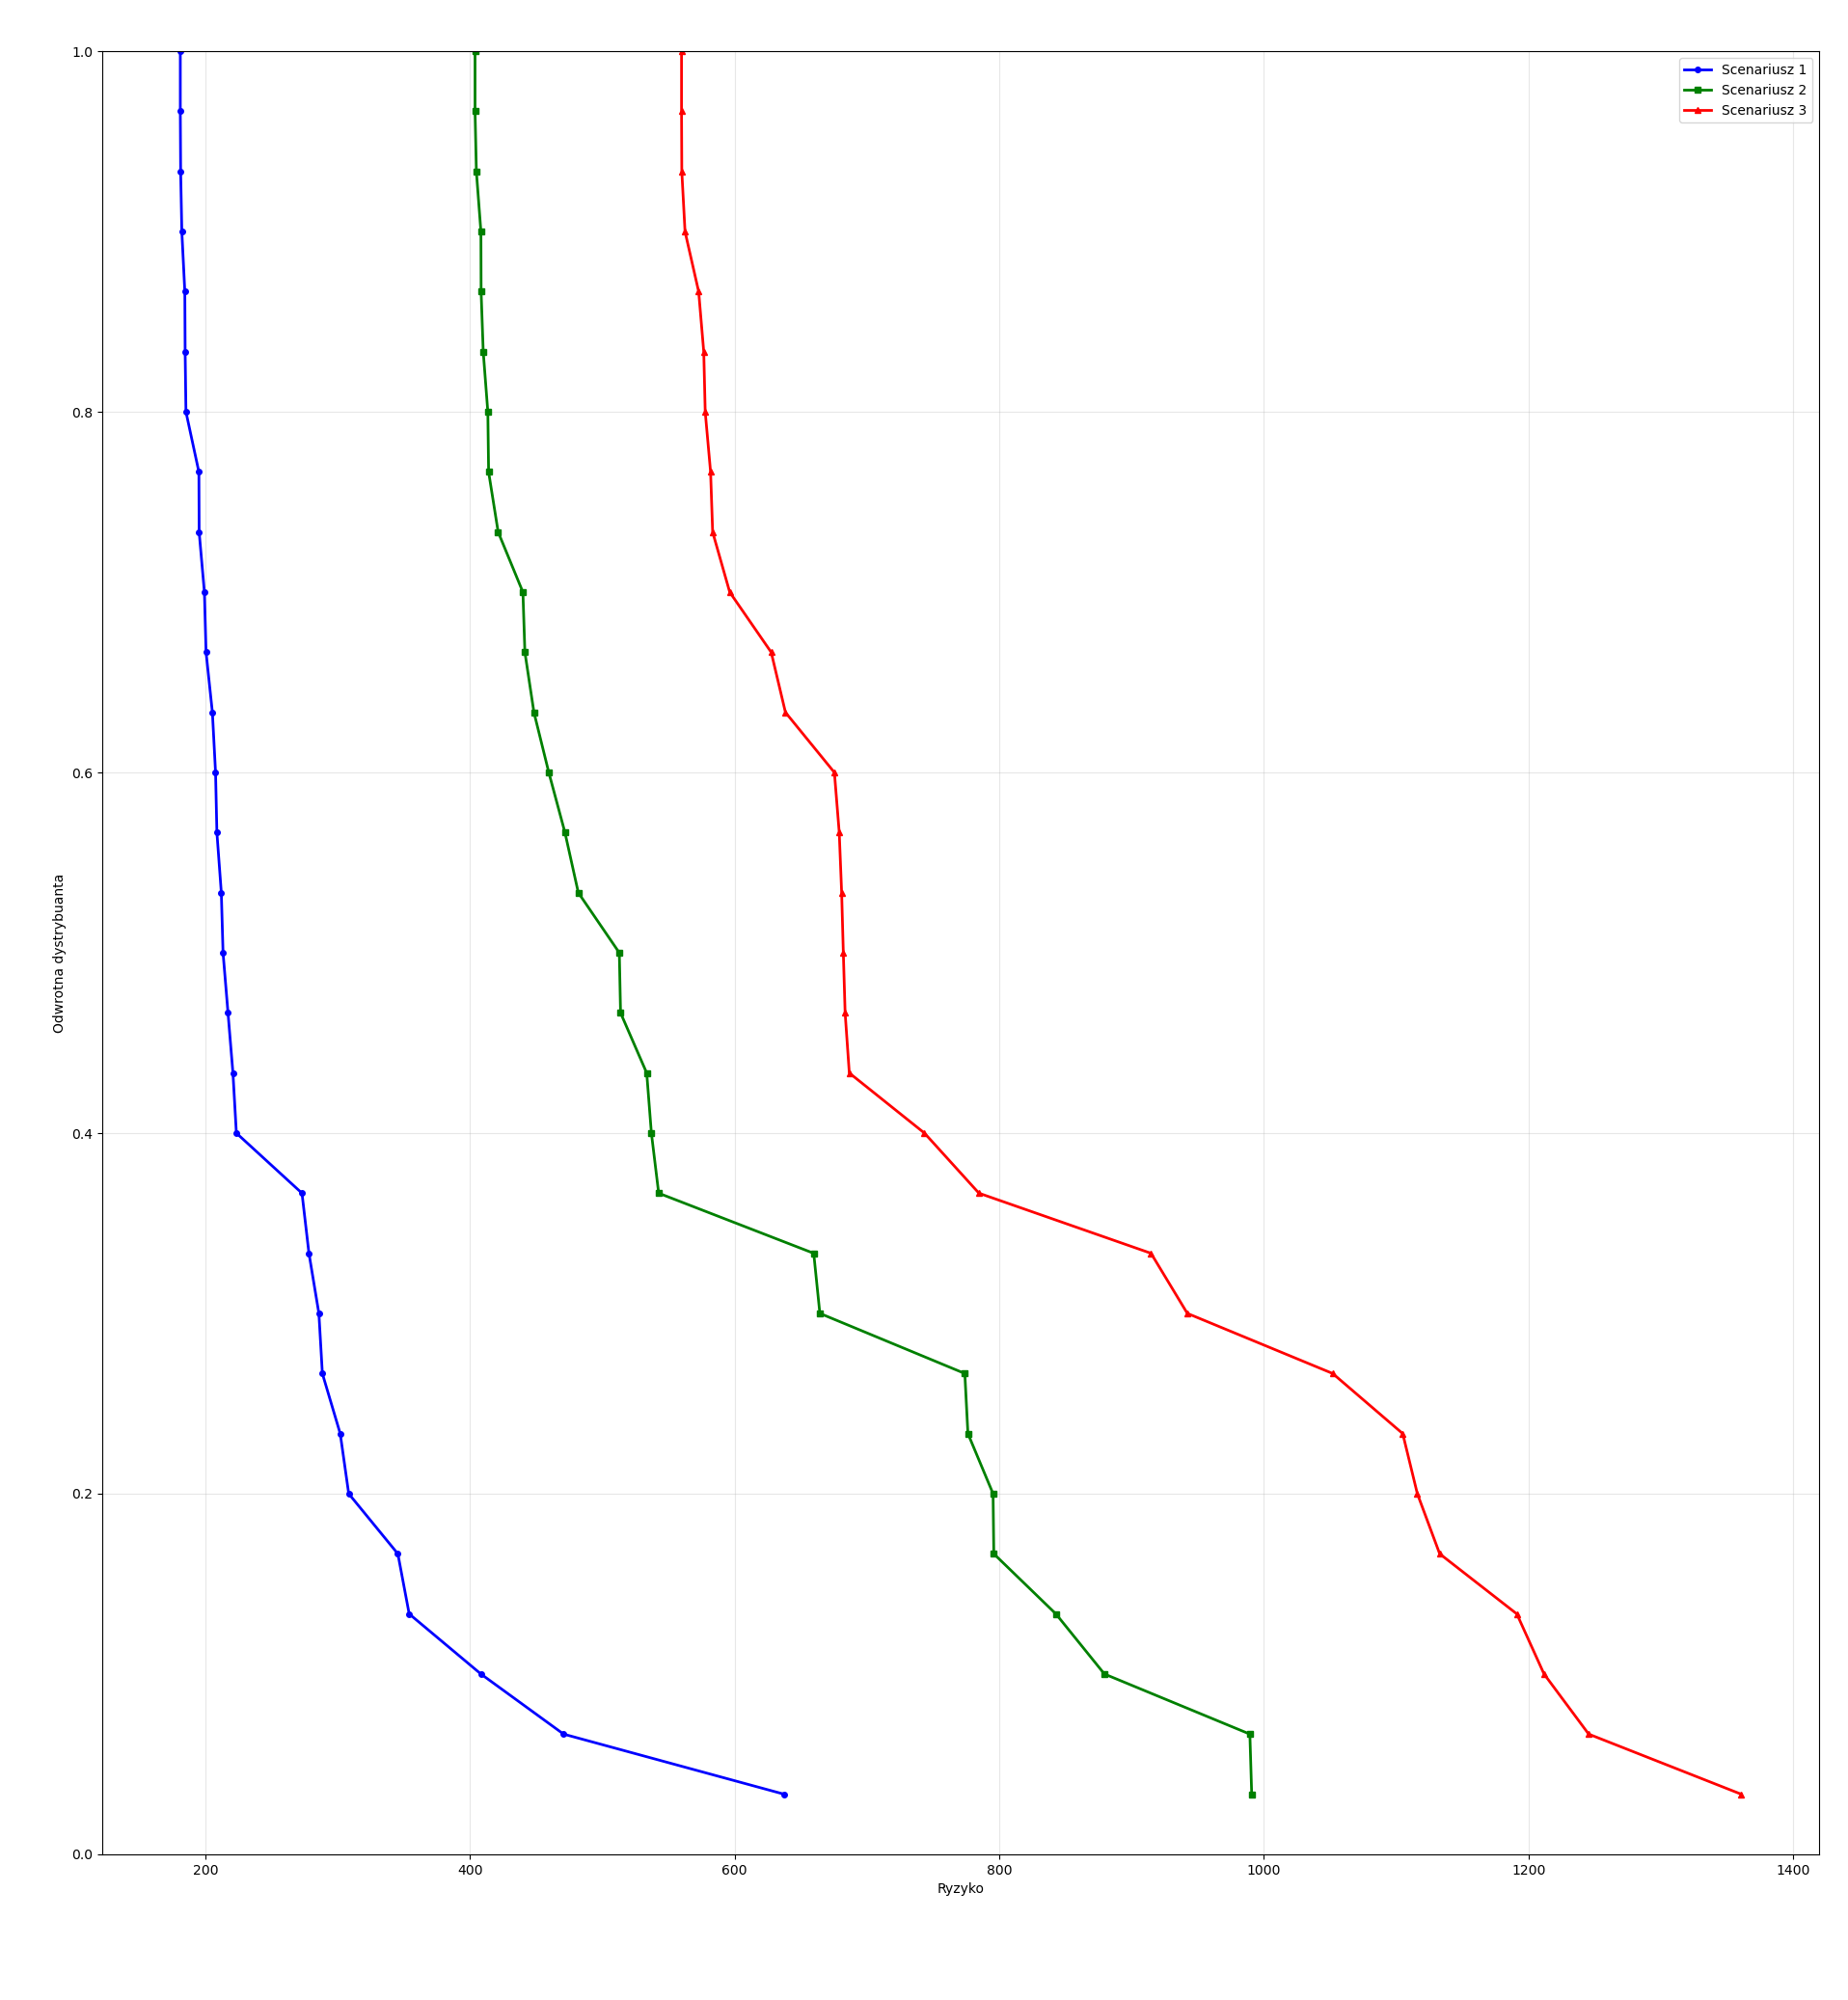
\includegraphics[width=\textwidth]{graphics/ryzyko_dystrybuanta.png}
\caption{Odwrotna dystrybuanta rozkładu średniej różnicy Giniego między scenariuszami}
\label{fig:FSD-risk}
\end{figure}


